\section{Theorie}

\subsection{Röntgenstrahlung}
Bei Röntgenstrahlung handelt es sich um hochenergetische elektromagnetische Wellen mit Wellenlängen unter $\SI{10}{\nano\meter}$. Diese kann
durch Abbremsung von beschleunigten Elektronen an einem bestimmten Material erzeugt werden. Dazu werden zunächst Elektronen in einer Glühkathode emittiert und über
eine Potentialdifferenz in einer evakuierten Röhre zu einer Anode beschleunigt, wo sie letztendlich abgebremst werden.
\\
Die Untersuchung des erzeugten Spektrums führt auf zwei unterschiedliche Komponenten, das kontinuierliche Bremsspektrum, sowie die charakteristische Röntgenstrahlung.
Das kontinuierliche Bremsspektrum entsteht bei Abbremsung der Elektronen im Coulomb-Potential der Atomkerne des Anodenmaterials. Dadurch entsteht jeweils ein Röntgenquant welches
 unterschiedliche Energien haben kann, je abhängig davon wie viel kinetische Energie das Elektron bei der Abbremsung verloren hat. Wenn das Elektron seine gesamte
Energie abgibt erhält das Photon die maximale Energie und es lässt sich eine minimale Wellenlänge angeben.
\\
\begin{align}
\nonumber
E_{\text{photon}} = E_{\text{kin}} \quad &\to \quad \frac{hc}{\lambda_{\text{min}}} = e U \\
&\to \quad \lambda_{\text{min}} = \frac{hc}{eU}
\end{align}
Dabei ist $h$ das Plancksche Wirkungsquantum, $c$ die Lichtgeschwindigkeit, $e$ die Elementarladung und $U$ die angelegte Spannung zwischen Kathode und Anode.
\\
Für den charakteristischen Strahlungsanteil muss das Anodenmaterial so ionisiert werden, dass eine Leerstelle auf einer inneren Schale entsteht. Anschließend kann ein Elektron einer höheren Schale diese Lücke füllen und geht
somit in ein geringeres Energieniveau über. Die Energiedifferenz resultiert in einer sehr spezifischen Wellenlänge des entstehenden Photons. Anders als bei der Bremsstrahlung sind diese Energiedifferenzen beim Übergang zwischen den
gleichen Energieniveuas immer äquivalent, wodurch scharfe Peaks im Spektrum entstehen.
\\
Die Energie der charakteristischen Strahlung lässt sich wie folgt ausdrücken.
\begin{equation}
\increment E = E_{m} - E_{n}
\end{equation}
Dabei deuten die Indizes auf die verschiedenen Energieniveus des Atoms hin. Dies gilt natürlich nur dann, wenn dieser Übergang der Niveaus auch den quantenmechanischen Auswahlregeln unterliegt.
\\
In einem Mehrelektronenatom schirmen die inneren Elektronen auf den unteren Schalen die Elektronen außen von dem Coulomb-Potential immer mehr ab. Das führt zu einer Verringerung der Bindungsenergie einzelnen Elektronen
auf äußeren Energieniveaus. Für die Bindungsenergie eines Elektrons auf der $n$-ten Schale gilt.
\begin{equation}
E_{n} = -R_{\infty} z_{\text{eff}}^{2} \cdot \frac{1}{n^{2}}
\end{equation}
Hierbei entspricht $R_{\infty}$ der bekannten Rydbergenergie von $\SI{13.6}{\electronvolt}$. Die effektive Kernladung $ z_{\text{eff}}$ ist folgendermaßen definiert.
\begin{equation*}
 z_{\text{eff}} = z - \sigma
\end{equation*}
Mit $z$ der Kernladung und $\sigma$ einer spezifischen Abschirmkonstante welche sich für jedes Elektron unterscheidet.
\\
Die Übergange der Energieniveaus besitzen eine bestimmte Notation. Ein Übergang welcher auf der ersten Schale endet bekommt den Buchstaben K, einer auf der zweiten Schale L, dies führt sich
alphabetisch fort. Nun wird ein Indize an diesen Buchstaben gesetzt, je nachdem von welchem Energieniveau das Elektron stammt. Hierbei wird bei $n=2$ gestartet und die Indizes bekommen
das griechische Alphabet zugewiesen für steigendes $n$.
In dem folgenden Versuch werden die Cu-$\text{K}_{\alpha}$ und Cu-$\text{K}_{\beta}$ Linien beobachtet.

\subsection{Absorption von Röntgenstrahlung}
Bei Röntgenstrahlung unter $\SI{1}{\mega\electronvolt}$ treten sehr häufig andere Effekte wie z.B der Compton-Effekt oder der Photoeffekt bei Bestrahlung eines Stoffes auf.
Die Absorption beschrieben durch den Absorptionskoeffizienten steigt mit abfallender Wellenlänge sprunghaft an. Dies geschieht immer dann wenn die Photonenergie gerade so groß ist, 
dass sie die Bindungsenergie der nächsten Schale des Stoffes trifft.
Diese Absorptionen zeichnen sich in einem Absorptionsdiagramm als scharfe Kanten aus, deshalb werden sie Absorptionskanten, z.B K${-}$,L${-}$ ... genannt.
\\
Aufgrund der Feinstrukturaufspaltung der Energieniveaus gibt es drei L-Kanten und eine K-Kante. In diesem Versuch wird lediglich die K-Kante einiger Stoffe untersucht.
Die Bindungsenergie $E_{n,j}$ eines Elektrons lässt sich gemäß der Sommerfeldschen Feinstrukturformel ermitteln. Dabei ist $n$ wieder die Energiequantenzahl und $j$ der Gesamtdrehimpuls welcher sich aus dem Bahndrehimpuls und dem
Spin des Elektrons zusammensetzt.
\begin{equation}
\label{eqn:sommerfeldenergie}
E_{n,j} = -R_{\infty} \left(z_{{{\text{eff}}^{2}}_{1}} \cdot \frac{1}{n^{2}} + {\alpha}^{2} z_{{{\text{eff}}^{2}}_{2}} \cdot \frac{1}{n^{3}} \left( \frac{1}{j + \frac{1}{2}} - \frac{3}{4n}\right)  \right)
\end{equation}
Das $\alpha$ steht für die Sommerfeldsche Feinstrukturkonstante. Elektronen aus der K-Schale besitzen die Energiequantenzahl $n = 1$ woraus sich zusammen mit der zuvor angegebenen Bindungsenergie \ref{eqn:sommerfeldenergie} eine
Abschirmkonstante bestimmen lässt.
\begin{equation}
\label{eqn:kackeq}
\sigma_{K} = Z - \sqrt{\frac{E_{K}}{R_{\infty}} - \frac{{\alpha}^{2}Z^{4}}{4}}
\end{equation}
Dieser berücksichtigt die Feinstrukturaufspaltung der Energieniveaus der K-Schale.

\subsection{Bragg´sche Reflexion}
Für die experimentelle Bestimmung der Wellenlänge der erzeugten Röntgenstrahlung kann ein Reflektionsverhalten an einem Kristallgitter verwendet werden.
Hierbei wird das Röntgenstrahlung auf ein dreidimensionales Gitter geschickt wobei jedes Photon an den Atomen des Kristalls gebeugt wird. Es entsteht ein Interferenzmuster mit einer bestimmten Eigenschaft.
Der Winkel $\theta$ unter dem konstruktive Interferenzmuster stattfindet wird Glanzwinkel genannt und bei bekannter Gitterkonstante lässt sich durch Winkelzusammenhänge folgende Bedingung aufschreiben.
Diese Bedingung wird auch Bragg´sche Bedingung genannt.
\begin{equation}
\label{eqn:lambda}
2 d \text{sin}(\theta) =  m \lambda \quad | m \in \mathbb{N}
\end{equation}
Hierbei ist $m$ ein ganze natürliche Zahl. Dies folgt aus der Voraussetzung für konstruktive Interferenz. Die Gitterkonstante $d$ ist dabei abhängig vom verwendeten Kristall.
Eine schematische Darstellung des Beugungsvorgangs ist in Abbildung \ref{fig:bild1} gezeigt.
\\
\begin{figure}[h]
  \centering
  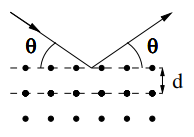
\includegraphics[width=0.3\textwidth]{bilder/bild1.png}
  \caption{Schematische Darstellung einer Reflexion am Kristall.}
  \label{fig:bild1}
\end{figure}
Über den Zusammenhang $E = h f$  und \ref{eqn:lambda} lässt sich die Bragg´sche Bedingung auch als Energie abhängig vom Winkel angeben (für $m=1$).
\begin{equation}
    \label{eqn:braggEnergy}
    E = \frac{h c}{2 d \sin (\theta )}
\end{equation}
Hier ist $h$ wieder das Plancksche Wirkungsquantum und $c$ die Lichtgeschwindigkeit.
